\section{Results}
\label{sec:results}

% I write the description of the plots in their caption. In a succesive step of the work we can move the plot descriptions in the text.

As said in the previous section, in the second part of the experiment we get two different kind of outputs, the first produced only by MC-SVM and the second produced by MC-SVM combined with HMM. In order to verify the quality of ours results we can compare them with the labels trasncribed by Harte, that we call $\mathcal{L}_{Harte}$. Given $\mathcal{L}_{SVM}$, $\mathcal{L}_{HMM}$ and $\mathcal{L}_{Harte}$ we can determine the obtained errors probabilities as shown in \eqref{eq:errorpart2}.

\begin{equation}
	P_{e} = \frac{\sum_{i=1}^{|\mathcal{L}_{Harte}|}\chi\{\mathcal{L}(i)==\mathcal{L}_{Harte}(i)\}}{|\mathcal{L}_{Harte}|}
	\label{eq:errorpart2}
\end{equation}



 In \ref{ta:resultbeforeHMM} we can look at the error probabilities obtained after the first step of testing, therefore before processing HMM. In \ref{tab:resultafterHMM} we can look at the results obtained after the second step of testing, therefore after processing HMM. In both cases we have different outputs depending on the testing rate $r_{test}$ and on the chosen extracted feature.

\begin{table}[h!]
	\caption{Error before processing HMM}
	\centering
	\begin{tabular}{|c |c c c|}
	\hline
	$r_{test}$ & CENS & CLP & CRP\\ \hline
	0.1 & 0.4946 & 0.4739 & 0.6206\\
	0.2 & 0.4657 & 0.6000 & 0.6376\\
	0.3 & 0.4765 & 0.5691 & 0.5803\\
	\hline
	\end{tabular}
	\label{tab:resultbeforeHMM}
\end{table}

\begin{table}[h!]
	\caption{Error after processing HMM}
	\centering
	\begin{tabular}{|c |c c c|}
	\hline
	$r_{test}$ & CENS & CLP & CRP\\ \hline
	0.1 & 0.4439 & 0.4502 & 0.5641\\
	0.2 & 0.4296 & 0.5919 & 0.5967\\
	0.3 & 0.4179 & 0.5484 & 0.5204\\
	\hline
	\end{tabular}
	\label{ta:resultafterHMM}
\end{table}

\begin{figure} [h!]
	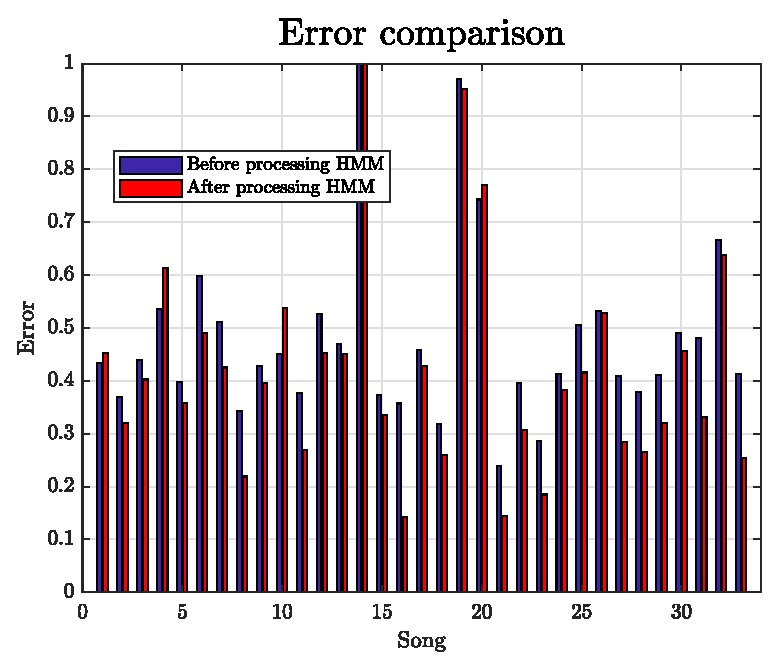
\includegraphics[width=0.5\textwidth]{img/Result_HMM/CENS/plot03071}
	\caption{Error comparison using CENS features (train = 0.7; test = 0.3). It is the one that has given the best results. We notice that a lot of songs have been discarded by Viterbi and therefore we have only 33 songs (not 150*0.3=45 as expected)}
\end{figure}

\begin{figure} [h!]
	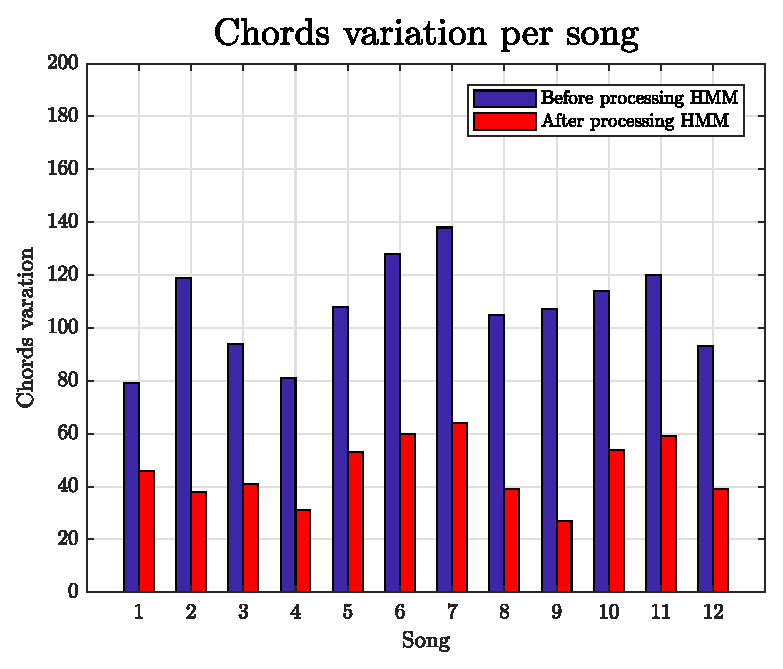
\includegraphics[width=0.5\textwidth]{img/Result_HMM/SMOOTHING/SmoothPerSongCENS0109}
	\caption{Chords variation per song using CENS features (train = 0.9; test = 0.1)}
\end{figure}

\begin{figure} [h!]
	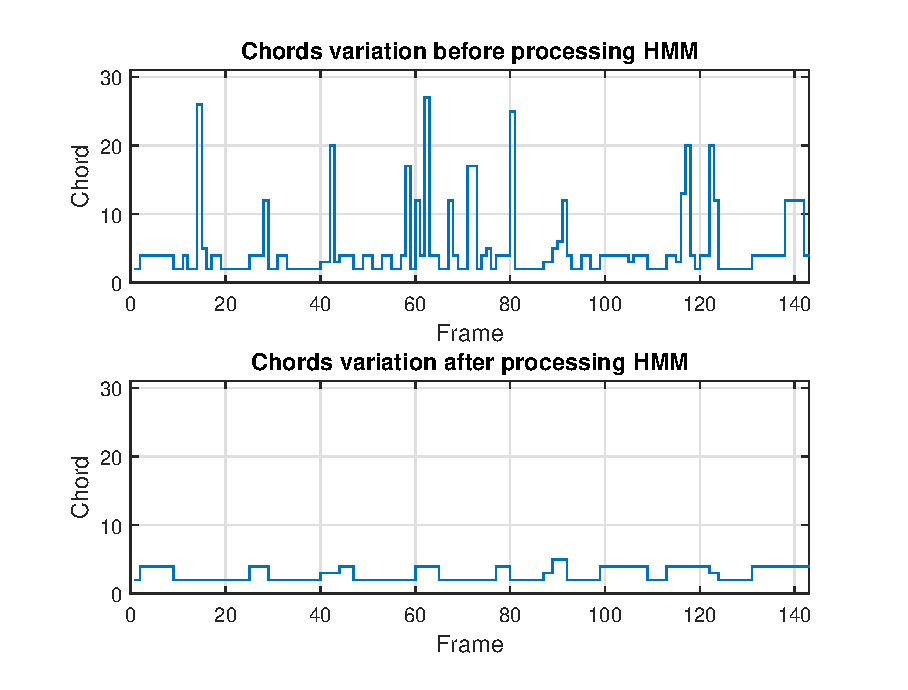
\includegraphics[width=0.5\textwidth]{img/Result_HMM/SMOOTHING/SmoothSingleSongCENS0109}
	\caption{Chord variation in a single song using CENS features (train = 0.9; test = 0.1); it represents the second song of the plot of the smoothing of all song}
\end{figure}
